\label{background}
\section{Sorting}

Sorting algorithms are used to arrange items consisting of \n{record}s and
\n{key}s. A key gives order to a collection of data called a record.  A real-life
example is a phone book: the records, phone numbers, are sorted by their keys,
names and addresses.

Sorts are frequently classified as \n{in-place} and \n{out-of-place}. An
out-of-place sort typically uses an extra array of the same size as the array to
be sorted. This may require the results to be copied back at the end. An
in-place sort does not require this extra array, though it may use a large
stack, especially in recursive algorithms.

A \n{stable} sort is one in which records which have the same key stay in the
same relative order during the sort. All the elementary sorts are stable, as are
mergesort and radixsort. Quicksort, heapsort and shellsort are not stable.

Sorting algorithms tend to be written using an \n{Abstract Data Type}, rather
than for a specific data type. This allows efficient reuse of the sorts, usually
as library functions. An example from the C standard library is the \cc{qsort}
function, which performs a sort on an arbitrary data type based on a comparative
function passed to it.

The ADT interface used here is taken from \cite{Sedgewick02}. An \cc{Item}
is a record, and a function is defined to extract its key.  Comparisons are done
via the \cc{less} function, and swapping is done using the \cc{exch} function.
These are replaced with their actual functions by the C preprocessor. The code
used for ADTs is in Figure \vref{Definitions used by the ADT}. The tests
presented in this report use \cc{unsigned integer}s as Items, which were
compared using a simple \n{less-than} function\footnote{This abstraction broke
down in several cases, such as where a \n{greater-than} function was required,
i.e. in quicksort.}.  In this case, a record and key are equivalent, and the
word \n{key} is used to refer to items to be sorted.

\code{Definitions used by the ADT}{adt.h}

There are special cases among sorts, where some sorts perform better on some
types of data. Most data to be sorted generally involves a small key.  This type
of data has low-cost comparisons and low-cost exchanges.  However, if strings
are being compared, then the comparison would have a much higher cost than the
exchange, since comparing keys could involved many comparisons - in the worst
case one on each letter. 

Sorts which are not comparison based also exist. These sorts are called counting
based sorts, as they count the number of keys to be put in each segment of an
array before putting them in place. The most important of these is radixsort,
discussed in Chapter \ref{radix}.

Sorts sometimes use a sentinel to avoid exceeding bounds of an array. If an
algorithm spends its time moving a key right based on a comparison with the key
next to it, then it will need to check that it doesn't go over the edge of the
array. This check, which can be expensive, can be replaced with a sentinel. This
is done by placing a maximal key off the right of the array, or by finding the
largest key in the array, and placing it in the final position. This technique
is used in quicksort and insertion sort.

\section{Caches}
Processors run many times faster than main memory. As a result, a processor
which must constantly wait for memory is not used to its full potential. To
overcome this problem, a \n{cache hierarchy} is used. A cache contains a small
subset of main memory in a smaller memory, which is much faster to access than
main memory. Modern computers typically contain many levels of cache, each with
increasing size and \n{latency}\footnote{Latency is the time between a request
being made and its successful execution.}. For example, it may take twice as
long to access the level 1 cache as it does to access a register. It may take
ten times as long as that to access the level 2 cache, and fifty times as long
to access main memory.

When a cache contains the data being sought, then this is called a cache
\n{hit}. When it does not, it is called a cache \n{miss}, and the next largest
cache in the hierarchy is queried for the data. There are three types of cache
miss: \n{compulsory} or \n{cold-start} misses, \n{conflict} misses and
\n{capacity} misses. A compulsory miss occurs when the data is first fetched
from memory. Since it has not been accessed before, it cannot already be in the
cache. A conflict miss occurs when the addressing scheme used by the cache
causes two separate memory locations to be mapped to the same area of the cache.
This only occurs in direct mapped or set-associative cache, described below.
Finally, a capacity miss occurs when the data sought has been ejected from the
cache due to a lack of space.

Caches range from direct mapped to fully associative. In a direct mapped cache,
every memory address has an exact position in the cache where it can be found.
Since the cache is smaller than main memory, many addresses map to the same position.
Fully associative is the opposite of this: data can be stored anywhere in the
cache. A set-associative cache is a mixture of both: more than one piece of data
can be stored in the same place. A 4-way set-associative cache allows four items
to be stored in the same place; when a fifth item needs to be stored in that
position, one of the items is ejected. The item may be ejected randomly, in a
specific order, or the \n{least recently used} item may be removed.

When data is loaded into the cache, data near it is loaded with it. This set of
data is stored in a \n{cache line} or \n{cache block}. The associativity and
length of the cache line dictate the mapping of memory addresses to cache
storage. Figure \vref{Addressing} shows how a memory address is divided.

\begin{figure}[h]
\centering
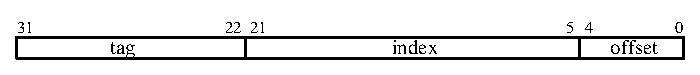
\includegraphics{cache_addressing}
\caption{Addressing}
\label{Addressing}
\end{figure}

This cache is a 2MB direct mapped cache.  There is a 32 byte cache line, which
is indexed by the 5 bit \n{offset}. There are $2^{16}$ cache lines, which are
indexed by the middle 16 bits of the address. The most significant 11 bits form
the \n{tag}. A cache line is tagged to check if the data stored at an index is
the same as the data requested. For a fully associative cache, there is no
index, and all the bits except the offset make up the tag. A fully associative
cache has no conflict misses for this reason; similarly, a direct mapped cache
has no capacity misses, since even when full, misses are due to conflicts.

The address used by the cache is not necessarily the address used by a program.
The addresses used within a program 
are called \n{virtual addresses}. Some caches are addressed by virtual address,
some caches by \n{physical address}, and some caches by \n{bus
address}\footnote{A bus address is used to address parts of the computer
connected over a bus, including main memory, multimedia controllers such as
sound and graphics cards, and storage devices such as hard drivers and floppy
disk controllers.}. Several optimizations in later chapters use the address to
offset arrays so that conflicts are not caused. However, because a program
cannot be sure of what type of addressing is used, the actual manipulated
address may not directly relate to the index used to address the cache. This
problem is not encountered in our simulations, as SimpleScalar
addresses its caches by virtual address.

Caches work on the principle of \n{locality}. It is expected that after some
data has been used once, it is likely to be used again in the near future. This
is called \n{\label{temporal locality}temporal locality}. Similarly, if some data is being used, it is
likely that data near it will also be used soon, such as two consecutive
elements of an array. This is called \n{spatial locality}. Many of the
algorithms presented here are designed to take advantage of locality. Spatial
locality is exploited by ensuring that once a cache line is loaded, each key in
the cache line is used. Temporal locality is exploited by ensuring that an
algorithm uses data as much as it can as soon as it is loaded, rather than over
a large time scale, during which it may have been ejected from the cache.

\section{Branch Predictors}

A branch is a conditional statement used to control the next instruction a
machine must execute. Typically, these are \cc{if} and \cc{while} statements,
or their derivatives. Branches cause delays in a processor's instruction
pipeline.  The processor must wait until the branch is resolved before it knows
what the next instruction is, and so it cannot fetch that instruction, and must
stall. To avoid this problem, modern processors use branch predictors, which
guess the branch direction and allow the processors to execute subsequent
instructions straight away.

Each branch can be resolved in two ways: \n{taken} or \n{not-taken}. If the branch is
taken, then the program counter moves to the address provided by the branch
instruction. Otherwise, the program counter increments, and takes the next
sequential instruction.

If a branch is mispredicted, then a long delay will occur, though this delay is
the same as if a branch predictor had not been used. During this delay, the
pipeline must be emptied, the instructions already executed must be discarded,
and the next instruction must be fetched.

In this report, we split branches into two types. The first is a \n{flow
control branch}. Flow control refers to controlling the flow of execution of a
program, and branches of this type are loops and other control statements.
The second type is a \n{comparative branch}: these are comparisons between two
pieces of data, such as two keys in an array being sorted. A branch can be both
a flow control and a comparative branch, but these will be referred to as
comparative branches here. This is due to the properties of the branches: a
comparative branch should not be easily predictable; a flow control branch
should be easy to predict based on previous predictions of the same branch.

There are several kinds of branch predictors: \n{static}, \n{semi-static} and
\n{dynamic}. This report only deals with dynamic predictors, which are of
interest due to their high accuracy. The other types are none-the-less discussed
below, as an introduction to dynamic predictors. A good discussion on predictor
types is \cite{Uht97}, from which the percentages below are taken. These
predictors were tested by Uht on the SPECint92 benchmarking suite. This is a
standard suite of integer-based programs used to measure the performance of an
architecture against another. Programs in this benchmark include \cc{gcc}, a
major C compiler, \cc{espresso}, which generates Programmable Logic Arrays and
\cc{li}, a LISP interpreter.

\subsection{Static Predictors}
A static predictor makes hardwired predictions, not based on information about
the program itself. Typically the processor will predict that branches are all
taken, or all not-taken, with 60\% and 40\% accuracy, respectively. Another type
of static branch predictor is Backwards-Taken-Forwards-Not-taken. Backward
branches are usually taken, so this increases the prediction accuracy to 65\%.

\subsection{Semi-static Predictors}
Semi-static predictors rely on the compiler to make their predictions for them.
The predictions don't change over the execution of a program, but the
improvement in predicting forward branches, which predominantly execute one way,
increases the accuracy to 75\%.

\subsection{Dynamic Predictors}
Dynamic predictors store a small amount of data about each branch, which
predicts the direction of the next branch. This data changes over the course of
a program's execution. Examples of this type of predictor are \n{1-bit},
\n{bimodal} and \n{two-level adaptive}.

\subsubsection{1-bit}
A 1-bit dynamic predictor uses a single bit to store whether a particular branch was last
taken or not-taken.  If there is a misprediction, then the bit is changed. 1-bit
predictors have the potential to mispredict every time, if the branch is
alternately taken and not taken. In the case of a loop with the sequence
T-T-T-N-T-T-T-N, a 1-bit predictor will mispredict twice per loop, or about half
the time.  Typically, though, it achieves an accuracy of 77 to 79\%.

\subsubsection{Bimodal}
A 2-bit dynamic predictor is called a bimodal predictor. It is a simple 2-bit
counter, each combination representing a state. In states 00 and 01, not-taken
is predicted; in states 10 and 11, taken is predicted. Each taken prediction
increments the count, to a maximum of 11, and each not-taken prediction
decrements the counter, to a minimum of zero.

In the sequence T-T-T-N-T-T-T-N, a 2-bit predictor will only mispredict once.
In general, it will achieve 78 to 89\% accuracy.

\subsubsection{Two-Level Adaptive}
A two-level adaptive predictor uses branch history to predict future branches. A
global branch history register keeps track of the last few branches, and uses
this to index a table of 2-bit predictors, which predict the result of the
branch. Frequently, the program counter is also included, either concatenated or
exclusive-ORed with the branch history to form the table index.

This type of predictor can predict the two cases above perfectly.  However, the
table can take time to fill, leading to cold-start misses, much like those of a
cache. Typically, a two-level adaptive predictor will be accurate 93\% of the time.

\section{Big O notation}
Big O notation is used to describe the complexity of an algorithm. It says that
the algorithm will complete in a certain number of steps, in relation to number
of items of data being worked on, without giving specifics of how many
instructions each step will take to execute. It is possible, therefore, that an
algorithm with a lower complexity will complete slower than an algorithm where
each step is executed very quickly, but which has a greater order of complexity.

Big O notation is used to describe how an algorithm scales. Doubling the number
of elements to be sorted by an $O(N)$ algorithm will roughly double the time it
takes to execute, but will quadruple the running time of an $O(N^2)$ algorithm.

An algorithm which is $O(N)$ is said to complete in linear time. An algorithm
which is $O(N^2)$ is said to complete in quadratic time.  $O(NlogN)$ algorithms
may take several orders of magnitude more time than $O(N)$ algorithms, and
typically use the \n{divide-and-conquer} principle, or use a binary tree to
reduce complexity. Quicksort, mergesort and heapsort are all of this type,
whereas elementary sorts, such as insertion sort, selection sort, bubblesort and
shakersort are $O(N^2)$ algorithms. Radixsort is $O(N)$, but can be more
expensive than quicksort, due to the cost of each step. These are discussed in
later chapters. The shellsort we use, called \n{Gonnet Shellsort} has a
complexity of TODO (see \ref{TODO}).

An important thing to note is that the time the algorithms take to execute are
proportion to their complexity, but different constants of proportionality are
used for different algorithms. An algorithm with $10N$ instructions is $O(N)$,
and is not differentiated from an algorithm with $1000N$ instructions by this
notation.
